\documentclass{article}
\renewcommand \thesection{\roman{section}}
\usepackage[utf8]{inputenc}
\usepackage{mathtools}
\usepackage{amsmath}
\usepackage{amsfonts}
\usepackage{amssymb}
\usepackage{graphicx}
\usepackage[margin=1in]{geometry}
\usepackage{multicol}
\usepackage{enumitem}
\setlist{nolistsep}
\setlength{\columnsep}{1cm}
\title{AP Physics Notes}
\begin{document}
  
  \begingroup  
    \centering
    \LARGE AP Physics Notes\\[1ex]
  \endgroup
  
  \section{Kinematics}
    \subsection{Position, Velocity, and Acceleration}
    	\begin{multicols}{2}
    		\[
            	\frac{d\vec{x}}{dt}=\vec{v}(t)
            \]
    		\[
            	\frac{d^2\vec{x}}{dt^2}=\frac{d\vec{v}}{dt}=\vec{a}(t)
            \]
    		\[
            	\bar{v}=\frac{\Delta{x}}{\Delta{t}}
            \]
    		\[
            	\bar{a}=\frac{\Delta{v}}{\Delta{t}}
            \]
    		\[
            	\vec{v_f}=\vec{v_i}+\vec{a}t
            \]
    		\[
            	\vec{d}=\vec{v_i}t+\frac{1}{2}\vec{a}t^2
            \]
    		\[
            	\vec{v_f}^2=\vec{v_i}^2+2\vec{a}(\Delta{x})
            \]
    		\[
            	g=-9.8\frac{m}{s^2}
            \]
    
    		\columnbreak
    
    		Freefall and Projectile Motion:
    		\vspace{3mm}
    		\begin{itemize}
    			\item All free-falling objects do not encounter air resistance\ldots in an ideal world
    			\item All free-falling objects (on Earth) accelerate downwards at a rate of approximately $9.8\frac{m}{s^2}$
    			\item All free-falling objects have a constant $v_x$
    			\item $v_y=0$ \ldots at maximum of y-value of projectile
    		\end{itemize}
    
    		\vspace{2ex}
    		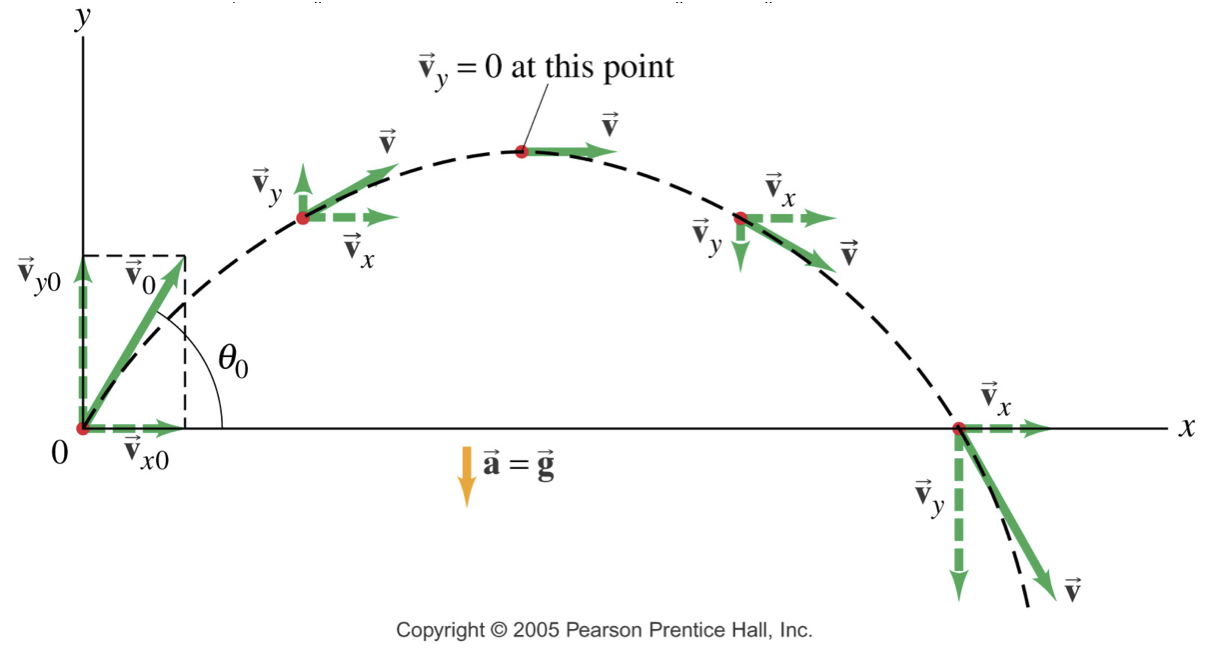
\includegraphics[width=8cm]{ProjectileMotion.jpg}
    	\end{multicols}
    \textbf{Sample Problems:}
    	\begin{multicols}{2}
    		A loose nail falls from the top of an elevator shaft.  At the same instant 25 m below is the roof of an elevator car rising at a constant 3.0 m/s. \\*\\* Find: \\*
    		\begin{enumerate}[label=\alph*]
    			\item Position \\*
    			\item Velocity of the nail just before it hits the roof of the elevator car\\*
    		\end{enumerate}
    		Nail: $v_i$ = 0$\frac{m}{s}$ and $d_y$ = 25m, above elevator\\*
    		Elevator: $v_i$ = 3$\frac{m}{s}$, up and $d_y$ = 0m
    
    		\columnbreak
    
    		\textit{In time, $t$, the vertical distance travelled equals:}
    		\[
            	\Delta{x_n}=25m-\frac{gt^2}{2} \indent \Delta{x_e}=0m-v_et
            \]
    
    		\textit{So, $t$ is the solution to the equation:}
    		\[
            	25m-\frac{gt^2}{2}=0m-v_et \indent t=1.9733s
            \]
    
    		\begin{enumerate}[label=\alph*]
    			\item $x=v_et=(-3\frac{m}{s})(1.9733s)=19m,$ up \\*
    			\item $v_n=gt=(-9.8\frac{m}{s^2})(1.9733s)=19\frac{m}{s},$ down
    		\end{enumerate}
    
    	\end{multicols}
    
    \noindent\centerline{\rule{5cm}{0.4pt}}
    
    	\begin {multicols}{2}
    		Suppose a volleyball player wants to serve the ball such that it just barely passes over the net.  Let x represent the horizontal distance to the net and y represent the height of the net relative to the launch point of the ball.
    		\\*\\*
    		Derive an equation that gives the initial launch angle in terms of x and y.
    	\columnbreak
    		\[
            	y=v_i\sin(\theta)t+\frac{at^2}{2} \indent x=v_i\cos(\theta)t
            \]
    		\[
            	v_i=\frac{y+\frac{gt^2}{2}}{t\sin(\theta)}=\frac{x}{t\cos(\theta)}
            \]
    		\[
            	y+\frac{gt^2}{2}=\frac{xt\sin(\theta)}{t\cos(\theta)}=xtan(\theta)
            \]
    		\[
            	y=\frac{gt^2}{2} \indent y+y=xtan(\theta) \indent \theta=tan^{-1}(\frac{2y}{x})
            \]
    	\end{multicols}
   	\noindent\centerline{\rule{10cm}{0.4pt}}
  \section{Dynamics}
  	\subsection{Newton's First Law of Motion}
  
  		Every object in a state of uniform motion tends to remain in that state of motion unless an external force is applied to it.
  		\\\\
  		\textbf{Inertia}: a property of matter by which it continues in its existing state of rest or uniform motion in a straight line, unless that state is changed by an external force.
  
  		\begin{multicols}{2}
  			\textbf{For instance} inertia is evident in the famous ``parlor trick'' where the  tablecloth is pulled from under the plates, tumblers, and silverware in a full dining setting. In this case the objects on the table are at rest, and, unless an external force is applied to each individual object, they will remain at rest. When the table cloth is pulled out from under the objects there are no significant external forces in play (friction is negligible if done correctly), and as a result only the tablecloth is removed.
  		\columnbreak
  			\centerline{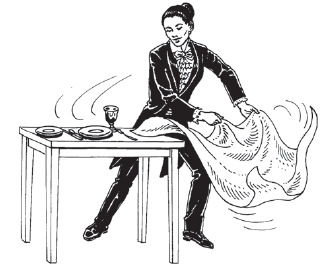
\includegraphics[width=5cm]{tableInertia.png}}
  		\end{multicols}
  
  	\subsection{Newton's Second Law of Motion}
  
  		The vector sum of the forces $\vec{F}$ on an object is equal to the mass $m$ of that object multiplied by the acceleration $\vec{a}$ of the object. $\vec{a}$ and $m$ are both directly proportional to $\vec{F}$. The $\vec{F}$ is the vector sum of all \emph{EXTERNAL} forces, so any internal interactions can be ignored.
  
  		\[
        	\Sigma\vec{F}=m\vec{a}
        \]
  
  	\subsection{Newton's Third Law of Motion}
  
  		When one body exerts a force on a second body, the second body simultaneously exerts a force equal in magnitude and opposite in direction on the first body.
  		\begin{multicols}{2}
  			\centerline{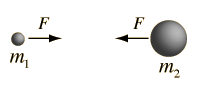
\includegraphics[width=6cm]{thirdLaw.png}}
  		\columnbreak
  			Without specifying the nature or origin of the forces on the two masses, Newton's 3rd law states that if they arise from the two masses themselves, they must be equal in magnitude but opposite in direction so that no net force arises from purely internal forces.
  		\end{multicols}
  
  	\subsection{Frictional Forces}
  
  		The weight of an object is defined as the force of gravity on the object and may be calculated as the mass times the acceleration of gravity.
  		\[
        	Weight=F_g=mg \indent g=9.8\frac{m}{s^2}
        \]
  
  		Frictional resistance to the relative motion of two solid objects is usually proportional to the force which presses the surfaces together as well as the roughness of the surfaces. Since it is the force perpendicular or ``normal'' to the surfaces which affects the frictional resistance, this force is typically called the ``normal force'' and designated by $F_N$.
  		\[
        	F_{friction}=\mu F_N
        \]
  		\begin{multicols}{2}
  			\noindent$F_N$ is the component of force perpendicular to the surface (surface being a plane) of contact.
  			\[
            	\mu_s>\mu_k
            \]
  			\centerline{$\mu_s$ -- Coefficient of static friction}\\*
  			\centerline{$\mu_k$ -- Coefficient of kinetic friction}
  		\columnbreak
  			\centerline{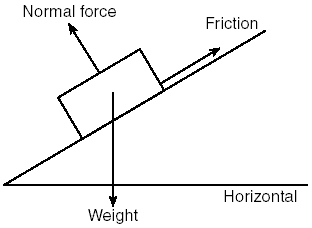
\includegraphics[width=4cm]{normalForce.png}}
  		\end{multicols}
  
  	\subsection{Atwood's Machine}
  		Frictionless and massless pulley:
  
  		\begin{multicols}{2}
  			\centerline{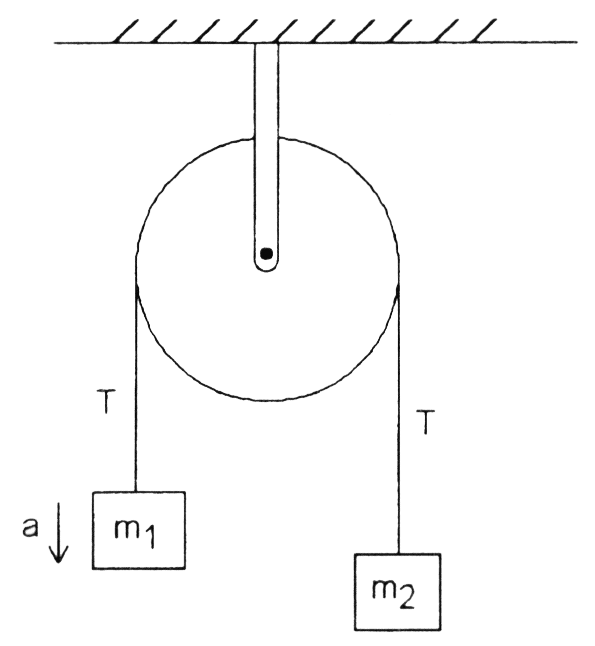
\includegraphics[width=3cm]{atwood.png}}
  		\columnbreak
  			\[
            	T=m_1g+\Sigma\vec{F}=m_1g+m_1\vec{a}=m_2g-m_2\vec{a}
            \]
  			\[
            	m_2g-m_1g-m_1\vec{a}=m_2\vec{a}
            \]
  			\[
            	\vec{a}=\frac{g(m_2-m_1)}{m_2+m_1}
            \]
  		\end{multicols}
  
  	\subsection{Air Resistance}
  		\textbf{Air resistance} is the result of collisions of the object's leading surface with air molecules, and it depends on the speed of the object and the cross-sectional area of the object. Eventually the force of air resistance equals the force of gravity, and prohibits any futher acceleration ($\vec{F_{net}}=0$). This state of freefall is called \textbf{terminal velocity}. Usually it is assumed that air resistance is proportional to speed or that it is proportional to the square of the speed (more accurate).
  		\[
        	\vec{F}_{D}\approx -k\vec{v} \indent or \indent \vec{F}_{D}\approx k\vec{v}^2
        \]
        Air Resistance is demonstrated in the following Position, Velocity, and Acceleration vs. Time graphs:\\
        \centerline{
  			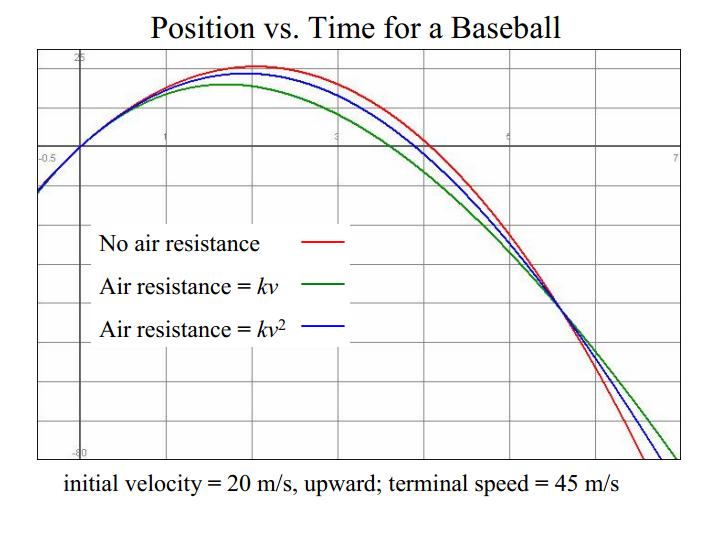
\includegraphics[width=5cm]{pvt_air.png}
        	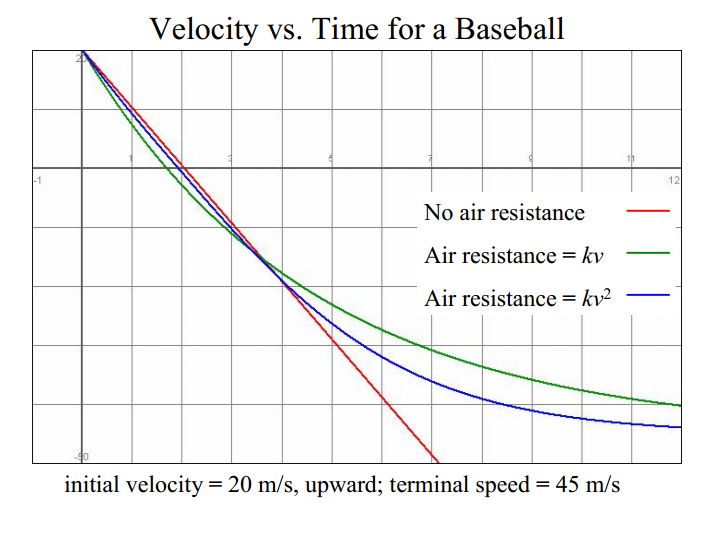
\includegraphics[width=5cm]{vvt_air.png}
        	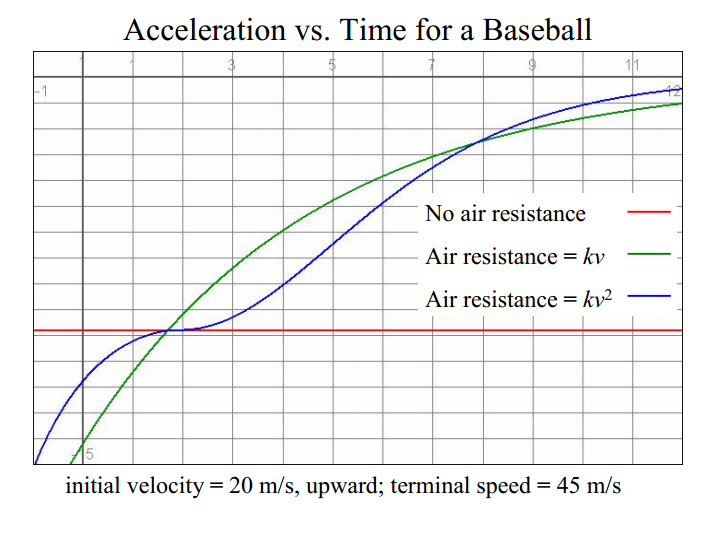
\includegraphics[width=5cm]{avt_air.png}
        }
  		\textbf{Sample Problems:}
        \begin{multicols}{2}
        Suppose a baseball of mass $m$ is falling through the air at a velocity $\vec{v}$ that is proportional to drag force $\vec{F}_D$. Solve for $\vec{v}$.
        \[
        	\Sigma\vec{F}=m\vec{a}=\vec{F}_g-\vec{F}_D=mg-k\vec{v}
        \]
        Guess and check method:
        \[
        	\vec{v}(t)=Ae^{Bt}+C \indent \vec{a}=\frac{d\vec{v}}{dt}=ABe^{Bt}
        \]
        \[
        	m\vec{a}=mg-k\vec{v} \indent m(ABe^{Bt})=mg-k(Ae^{Bt}+C)
        \]
        \[
        	mABe^{Bt}=mg-kAe^{Bt}-kC
        \]
        \columnbreak
        \[
        	0=mg-kC \indent mg=kC \indent C=\frac{mg}{k} \indent \text{(C)}
        \]
        \[
        	mABe^{Bt}=-kAe^{Bt} \indent mB=-k \indent B=\frac{-k}{m} \indent \text{(B)}
        \]
        \[
        	\vec{v}(t)=Ae^{Bt}+C=Ae^{-kt}{m}+\frac{mg}{k}
        \]
        \[
        	\vec{v}(0)=Ae^{-k(0)}{m}+\frac{mg}{k} \indent A=\frac{-mg}{k} \indent \text{(A)}
        \]
        \[
        	\therefore \indent \vec{v}(t)=\frac{mg}{k}(1-e^{\frac{-kt}{m}})
        \]
        \end{multicols}
        
        \noindent\centerline{\rule{5cm}{0.4pt}}
  		
        \begin{multicols}{2}
  			Must an object always move in the direction of the net force acting upon it?  Explain and give examples to support your answer.
  			\vfill
  		\columnbreak
  			\textit{No, an object doesn't necessarily have to move in the direction of the $\vec{F}_{net}$. An example is circular motion, where the $\vec{F}_{net}$ is towards the center.}
  		\end{multicols}
  
  		\noindent\centerline{\rule{5cm}{0.4pt}}
  
  		\begin{multicols}{2}
  			A cart on wheels is loaded with books.  In order to move the cart you must exert a relatively great force to start it moving but then a much smaller force to keep it moving.  Use Newton’s laws to explain.
  			\vfill
  		\columnbreak
  			\textit{An object at rest has the tendency to remain at rest, and so the cart loaded with books (when at rest) wants to remain in it's state of rest. Thus, in order to move it one must exert a greater force than the force required to keep the cart in motion.}
  		\end{multicols}
  
  		\noindent\centerline{\rule{5cm}{0.4pt}}
  
  		\begin{multicols}{2}
  			A pair of fuzzy dice hangs from the ceiling of a car that accelerates forward at $3.00\frac{m}{s^2}$.  Assuming the dice have the same acceleration as the car, what is the angle $\theta$ as shown in the diagram below?\\\\
  			\centerline{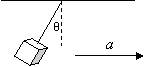
\includegraphics[width=5cm]{dice.png}}
  		\columnbreak
  			\[
            	\Sigma\vec{F}=m\vec{a}=\vec{T}\sin(\theta)
            \]
  			\[
            	\vec{T}\cos(\theta)=mg \indent \vec{T}=\frac{mg}{\cos(\theta)}
            \]
  			\[
            	m\vec{a}=\frac{mg\sin(\theta)}{\cos(\theta)}
            \]
  			\[
            	\frac{\vec{a}}{g}=tan(\theta)
            \]
  			\[
            	\theta=tan^{-1}\frac{\vec{a}}{g}=tan^{-1}(\frac{3.00\frac{m}{s^2}}{9.8\frac{m}{s^2}})=17.02^{\circ}
            \]
  		\end{multicols}
  
  		\noindent\centerline{\rule{5cm}{0.4pt}}
  
  		\begin{multicols}{2}
  			As shown in the diagram below, two blocks are connected by a lightweight cord that passes over a frictionless, massless pulley.  The bottom block has a mass of $2.00 kg$ and the top block has mass $0.500 kg$.  The coefficient of kinetic friction at each sliding surface is equal to $0.10$.  The two blocks are release from rest.  Determine the acceleration, $\vec{a}$, of each block.
  			\centerline{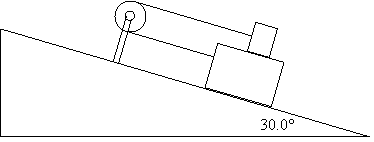
\includegraphics[width=6cm]{frictionPlane.png}}
  			\vfill
  		\columnbreak
  			\noindent\textit{Net force for $m_1$ (smaller block):}
  			\[
            	\Sigma\vec{F}=m_1\vec{a}=T-m_1 g\sin(\theta)-\mu_km_1g\cos(\theta)
            \]
  			\textit{Net force for $m_2$ (larger block):}
  			\[
            	\Sigma\vec{F}=m_2\vec{a}=m_2g\sin(\theta)-T-\mu_km_1g\cos(\theta)-\mu_k(m_1+m_2)g\cos(\theta)
            \]
            
       	\end{multicols}
  
  		\noindent\centerline{\rule{10cm}{0.4pt}}
  
  \section{Circular Motion and Gravity}
  
  	\subsection{Uniform Circular Motion}
  		Anything in circular motion is always accelerating towards the center, this value is called centripetal acceleration. Centripetal means ``center-seeking''. Velocity in circular motion is directed tangential to the circular path of the object.
  		\begin{multicols}{2}
        	\centerline{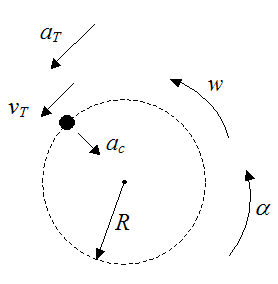
\includegraphics[width=5cm]{circularMotion.png}}
            \columnbreak
  			\[
            	\vec{v}=\frac{2\pi r}{T}
            \]
  			\[
            	\vec{a}=\frac{v^2}{r}
            \]
  			\[
            	\Sigma\vec{F}=m(\vec{a})=\frac{mv^2}{r}
            \]
            \[
            	f=\frac{1}{T}
            \]
      	\end{multicols}
  	\subsection{Non-uniform Circular Motion}
    	Non-uniform circular motion is any case in which an object moving in a circular path has a varying speed. The tangential acceleration is non-zero; the speed is changing.The net acceleration is no longer pointing towards the center, so there are two components of acceleration that we would need to account for:\vspace{1ex}
        \begin{multicols}{2}
        	\begin{enumerate}
        		\item Radial/centripetal acceleration ($a_R$)
            	\item Tangential acceleration ($a_\theta$)
        	\end{enumerate}
            \centerline{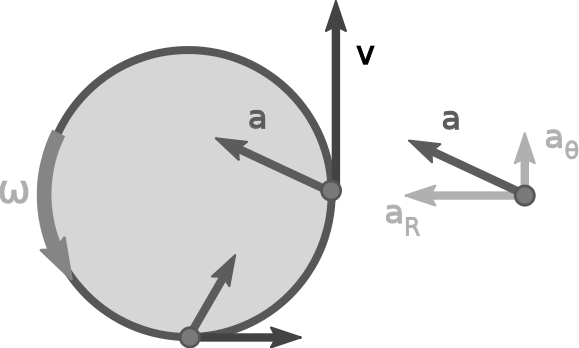
\includegraphics[width=6cm]{noncirc.png}}
       	\columnbreak
        	\[
            	\lvert\vec{a}\rvert=\sqrt{\vec{a_\theta}^2+\vec{a_R}^2}
            \]
        	\noindent{Suppose centripetal force was denoted $\vec{T}$, then:}
            \[
            	\vec{T}-mg\cos(\theta) = m\vec{a}_R = \frac{m\vec{v}^2}{r} \indent \text{(Radial Dir.)}
            \]
            \[
            	mg\sin(\theta)=m\vec{a}_\theta \indent \text{(Tangential Dir.)}
            \]
            We note that velocity, tangential acceleration and tangential force all act along the same direction.
            \[
            	\vec{a}_\theta=\frac{d\vec{v}}{dt}
            \]
        \end{multicols}
        
\end{document}